% Provenance (never printed): cycle 4 (geographie and SVT, "La planete Terre"):
% why a flat map distorts, projections, scale, topographic maps and
% profiles, satellite images and satellite positioning; see
% sources/book1/PROVENANCE.md. Book 1, grade 9, chapter 5.
% Vocabulary guard: owns map projection (Mercator, equal-area), numerical
% scale and scale bar, topographic map, contour line and contour interval,
% remote sensing and satellite image, satellite positioning. "Scale" itself
% is g2's (drawing-to-map, Sync 1 ruling); globe and world map are g3's;
% parallels, meridians, latitude and longitude are g6's; altitude, relief
% and physical map are g4's; slope as a percentage was used in g9.2. The
% speed of light is the physics books' (recalled in prose). The V-rule of
% geological maps belongs to Book 3.
\chapter{Peta Seluruh Bumi}\label{ch:g9:maps-of-the-earth}

Pada banyak \omterm{def:g2:drawing-to-map:map}{peta} dinding di kelas, Greenland tampak hampir sebesar Afrika.
Pada \omterm{def:g3:continents-and-oceans:globe}{bola dunia}, Afrika sekitar empat belas kali lebih luas: sekitar
29~juta kilometer persegi untuk daratan utama Afrika, dibandingkan dengan
sekitar 2.1~juta untuk Greenland. Keduanya adalah gambaran Bumi yang
jujur, dibuat dengan cermat. Lalu, mana yang berbohong, dan mengapa?
% ledger: data:ne-land (areas computed in figdata/grade-9/projections.py)

\begin{recall}
\omterm{def:g2:drawing-to-map:map}{Peta} adalah gambar suatu tempat yang dilihat dari atas, lebih kecil
daripada tempat itu, dengan \omterm{def:g2:drawing-to-map:legend}{legenda} dan \omterm{def:g2:drawing-to-map:scale}{skala}
(\cref{ch:g2:drawing-to-map}). \omterm{def:g3:continents-and-oceans:globe}{Bola dunia} adalah model kecil Bumi yang
bulat; \omterm{def:g3:continents-and-oceans:world-map}{peta dunia} menampilkan seluruh Bumi secara datar, dalam satu gambar
(\cref{ch:g3:continents-and-oceans}). \omterm{def:g6:latitude-longitude:latitude}{Paralel} dan \omterm{def:g6:latitude-longitude:longitude}{meridian} memberi setiap
tempat \omterm{def:g6:latitude-longitude:latitude}{lintang} dan \omterm{def:g6:latitude-longitude:longitude}{bujurnya} (\cref{ch:g6:latitude-longitude}). \omterm{def:g4:world-physical-map:altitude}{Ketinggian}
adalah tinggi di atas \omterm{def:g4:world-physical-map:altitude}{permukaan laut}, dan \omterm{def:g4:world-physical-map:physical-map}{peta fisik} menampilkan \omterm{def:g4:world-physical-map:relief}{relief}
dengan warna-warna (\cref{ch:g4:world-physical-map}). Dalam fisika, kamu
mempelajari bahwa cahaya merambat sekitar \qty{300000}{km} per detik.
\end{recall}
% ledger: const:c

\section{Mengapa peta datar pasti mengubah bentuk}

Cobalah meratakan kulit jeruk di atas meja: kulit itu robek atau
meregang. Permukaan bola tidak dapat dibentangkan datar tanpa mengubah
sebagian panjangnya. Untuk menggambar seluruh Bumi pada selembar kertas,
pembuat \omterm{def:g2:drawing-to-map:map}{peta} memilih suatu aturan yang memindahkan setiap titik \omterm{def:g3:continents-and-oceans:globe}{bola dunia}
ke satu titik pada kertas, dan memilih apa yang akan tetap benar pada \omterm{def:g2:drawing-to-map:map}{peta},
serta apa yang akan dikorbankannya.

\begin{definition}[Proyeksi peta]\label{def:g9:maps-of-the-earth:projection}
Yang disebut \emph{proyeksi peta}\index{proyeksi peta} adalah aturan yang
memindahkan setiap titik \omterm{def:g3:continents-and-oceans:globe}{bola dunia}, yang ditentukan oleh \omterm{def:g6:latitude-longitude:latitude}{lintang} dan
\omterm{def:g6:latitude-longitude:longitude}{bujurnya}, ke satu titik pada \omterm{def:g2:drawing-to-map:map}{peta} datar. Pada \emph{proyeksi
Mercator}\index{proyeksi Mercator}, \omterm{def:g6:latitude-longitude:latitude}{paralel} dan \omterm{def:g6:latitude-longitude:longitude}{meridian} berupa garis
lurus yang saling berpotongan tegak lurus, dan bentuk setiap wilayah kecil
tetap terjaga, tetapi luasnya makin diperbesar ke arah \omterm{def:g3:continents-and-oceans:poles}{kutub}. Pada
\emph{proyeksi sama luas}\index{proyeksi sama luas}, setiap wilayah tetap
mempunyai luas yang benar dibandingkan dengan wilayah lain, tetapi
bentuknya terdistorsi, makin kuat ke arah tepi \omterm{def:g2:drawing-to-map:map}{peta}.
\end{definition}

Gambar di bawah ini memindahkan lingkaran-lingkaran yang sama, semuanya
berukuran sama pada \omterm{def:g3:continents-and-oceans:globe}{bola dunia}, ke kedua \omterm{def:g2:drawing-to-map:map}{peta}. Pada \omterm{def:g2:drawing-to-map:map}{peta} Mercator,
lingkaran-lingkaran itu tetap bulat tetapi membesar ke arah \omterm{def:g3:continents-and-oceans:poles}{kutub}: pada
\omterm{def:g6:latitude-longitude:latitude}{lintang} \ang{60}, luasnya empat kali luasnya di \omterm{def:g3:continents-and-oceans:equator}{khatulistiwa}, dan di
dekat bagian tengah Greenland, pada sekitar \ang{72}, sekitar sepuluh kali.
Pada \omterm{def:g2:drawing-to-map:map}{peta} sama luas, semua lingkaran itu tetap mempunyai luas yang sama,
tetapi lingkaran yang jauh dari pusat \omterm{def:g2:drawing-to-map:map}{peta} tergencet menjadi lonjong.
% ledger: data:ne-land (circles and factors computed in figdata/grade-9/projections.py, mercator_area_factor)

Tidak ada proyeksi yang terbaik untuk segala keperluan. \omterm{def:g9:maps-of-the-earth:projection}{Proyeksi Mercator}
dibuat untuk pelaut: haluan yang mempertahankan arah kompas yang sama
tampak sebagai garis lurus pada \omterm{def:g2:drawing-to-map:map}{peta} itu. Untuk membandingkan luas
negara, hutan, atau \omterm{def:g5:weather-and-climate:desert}{gurun}, \omterm{def:g2:drawing-to-map:map}{peta} sama luaslah yang menunjukkan kebenaran.
Sebelum memercayai sebuah \omterm{def:g3:continents-and-oceans:world-map}{peta dunia}, ada baiknya kita bertanya proyeksi
apa yang dipakainya.

\begin{omfigure}
\begin{tikzpicture}
\begin{axis}[name=merc, x=0.0215cm, y=0.0215cm, xmin=-180, xmax=180,
  ymin=-140, ymax=169, axis line style={black!50}, ticks=none,
  title={\footnotesize proyeksi Mercator}, title style={yshift=-1ex}]
  \addplot[black!15, line width=0.3pt] table {figdata/out/grade-9-projections-merc-grid.dat};
  \addplot[fill=black!25, draw=black!45, line width=0.15pt] table {figdata/out/grade-9-projections-merc-land.dat};
  \addplot[fill=orange!55, draw=orange!70!black, line width=0.3pt] table {figdata/out/grade-9-projections-merc-greenland.dat};
  \addplot[fill=blue!30, draw=blue!60!black, line width=0.3pt] table {figdata/out/grade-9-projections-merc-africa.dat};
  \addplot[red!80!black, line width=0.6pt] table {figdata/out/grade-9-projections-merc-circles.dat};
\end{axis}
\begin{axis}[at={(merc.east)}, anchor=west, xshift=0.3cm, x=0.025cm, y=0.025cm,
  xmin=-165, xmax=165, ymin=-83, ymax=83, hide axis,
  title={\footnotesize sebuah proyeksi sama luas}, title style={yshift=-1ex}]
  \addplot[black!15, line width=0.3pt] table {figdata/out/grade-9-projections-moll-grid.dat};
  \addplot[fill=black!25, draw=black!45, line width=0.15pt] table {figdata/out/grade-9-projections-moll-land.dat};
  \addplot[fill=orange!55, draw=orange!70!black, line width=0.3pt] table {figdata/out/grade-9-projections-moll-greenland.dat};
  \addplot[fill=blue!30, draw=blue!60!black, line width=0.3pt] table {figdata/out/grade-9-projections-moll-africa.dat};
  \addplot[red!80!black, line width=0.6pt] table {figdata/out/grade-9-projections-moll-circles.dat};
\end{axis}
\end{tikzpicture}

{\small Dunia yang sama pada dua proyeksi. Merah: lingkaran-lingkaran yang
berukuran sama pada \omterm{def:g3:continents-and-oceans:globe}{bola dunia}, berpusat setiap \ang{30} \omterm{def:g6:latitude-longitude:latitude}{lintang} dan
\ang{60} \omterm{def:g6:latitude-longitude:longitude}{bujur}. Jingga: Greenland; biru: daratan utama Afrika. Pada \omterm{def:g2:drawing-to-map:map}{peta}
Mercator (kiri, dipotong pada \ang{80}\,LS dan \ang{84}\,LU, karena \omterm{def:g3:continents-and-oceans:poles}{kutub}
akan terletak jauh tak terhingga), keduanya tampak hampir sama besar; pada
\omterm{def:g2:drawing-to-map:map}{peta} sama luas (kanan), Afrika sekitar 14 kali lebih luas, seperti pada
\omterm{def:g3:continents-and-oceans:globe}{bola dunia}. Garis pantai dari Natural Earth.}
% ledger: data:ne-land
\label{fig:g9:maps-of-the-earth:projections}
\end{omfigure}

\begin{example}[Greenland dan Afrika]
Daratan utama Afrika meliputi sekitar 29~juta~\unit{km^2}, Greenland
sekitar 2.1~juta~\unit{km^2}: $29 \div 2.1 \approx 14$. Afrika terbentang
di kedua sisi \omterm{def:g3:continents-and-oceans:equator}{khatulistiwa}, tempat \omterm{def:g9:maps-of-the-earth:projection}{proyeksi Mercator} hampir tidak
memperbesar apa pun, sedangkan sebagian besar Greenland terletak di antara
sekitar \ang{60} dan \ang{84} \omterm{def:g6:latitude-longitude:latitude}{lintang} utara, tempat luas diperbesar 4
sampai lebih dari 10 kali. Pada \omterm{def:g2:drawing-to-map:map}{peta} Mercator, keduanya tampak hampir sama
besar.
\end{example}
% ledger: data:ne-land (areas and ratios computed in figdata/grade-9/projections.py, areas)

\section{Skala}

\omterm{def:g2:drawing-to-map:map}{Peta} sebuah \omterm{def:g1:landscapes-around-us:landform}{lembah} atau sebuah kota mencakup bagian Bumi yang begitu kecil
sehingga proyeksinya hampir tidak berpengaruh. Yang penting adalah berapa
kali \omterm{def:g2:drawing-to-map:map}{peta} itu lebih kecil daripada keadaan di lapangan.

\begin{definition}[Skala angka dan batang skala]\label{def:g9:maps-of-the-earth:numerical-scale}
Yang disebut \emph{skala angka}\index{skala angka} sebuah \omterm{def:g2:drawing-to-map:map}{peta} adalah
perbandingan seperti $1 : 25\,000$: satu sentimeter pada \omterm{def:g2:drawing-to-map:map}{peta} mewakili
\num{25000} sentimeter di lapangan, dan begitu pula untuk satuan apa pun.
Yang disebut \emph{batang skala}\index{batang skala} adalah penggaris yang
digambar pada \omterm{def:g2:drawing-to-map:map}{peta}, yang diberi tanda jarak-jarak di lapangan.
\end{definition}

\begin{method}[Memakai skala angka]
\begin{enumerate}
  \item Ukurlah jarak pada \omterm{def:g2:drawing-to-map:map}{peta}, dalam sentimeter.
  \item Kalikan jarak itu dengan bilangan di belakang titik dua: hasilnya
        adalah jarak di lapangan, dalam sentimeter.
  \item Ubahlah satuannya: bagi dengan 100 untuk meter, dengan
        \num{100000} untuk kilometer.
\end{enumerate}
\end{method}

\begin{example}[Berjalan kaki pada peta $1 : 25\,000$]
Pada \omterm{def:g2:drawing-to-map:map}{peta} berskala $1 : 25\,000$, sebuah jalan setapak panjangnya
\qty{6}{cm}. Di lapangan, panjangnya $6 \times 25\,000 = \num{150000}$~cm,
yaitu \qty{1500}{m} atau \qty{1.5}{km}. Setiap sentimeter pada \omterm{def:g2:drawing-to-map:map}{peta}
mewakili \qty{250}{m}.
\end{example}

\omterm{def:g9:maps-of-the-earth:numerical-scale}{Batang skala} mempunyai satu kelebihan dibandingkan dengan \omterm{def:g9:maps-of-the-earth:numerical-scale}{skala angka}:
ketika \omterm{def:g2:drawing-to-map:map}{peta} diperbesar atau diperkecil pada layar atau mesin fotokopi,
batang itu ikut diperbesar atau diperkecil sehingga tetap benar,
sedangkan perbandingan yang tercetak di sudut \omterm{def:g2:drawing-to-map:map}{peta} menjadi salah.

\section{Peta topografi}

\omterm{def:g4:world-physical-map:physical-map}{Peta fisik} menunjukkan \omterm{def:g4:world-physical-map:relief}{relief} dengan warna-warna. \omterm{def:g2:drawing-to-map:map}{Peta} suatu daerah kecil
menunjukkannya jauh lebih teliti, dengan garis-garis.

\begin{definition}[Peta topografi]\label{def:g9:maps-of-the-earth:topographic-map}
Yang disebut \emph{peta topografi}\index{peta topografi} adalah \omterm{def:g2:drawing-to-map:map}{peta}
terperinci suatu daerah kecil, dengan \omterm{def:g2:drawing-to-map:scale}{skala} seperti $1 : 25\,000$ atau
$1 : 50\,000$, yang menunjukkan bentuk dan \omterm{def:g4:world-physical-map:altitude}{ketinggian} permukaan tanah,
beserta \omterm{def:g1:landscapes-around-us:water}{sungai}, jalan raya, jalan setapak, bangunan, dan hutan.
\end{definition}

\begin{definition}[Garis kontur dan interval kontur]\label{def:g9:maps-of-the-earth:contour}
Yang disebut \emph{garis kontur}\index{garis kontur} adalah garis pada
\omterm{def:g2:drawing-to-map:map}{peta} yang menghubungkan titik-titik permukaan tanah yang sama
\omterm{def:g4:world-physical-map:altitude}{ketinggiannya}. Yang disebut \emph{interval kontur}\index{interval kontur}
adalah selisih \omterm{def:g4:world-physical-map:altitude}{ketinggian} antara dua garis kontur yang bersebelahan;
nilainya sama di seluruh \omterm{def:g2:drawing-to-map:map}{peta}.
\end{definition}

Bayangkan sebuah \omterm{def:g1:landscapes-around-us:landform}{bukit} yang diiris oleh bidang-bidang mendatar, satu
setiap \qty{100}{m}. Setiap irisan memotong \omterm{def:g1:landscapes-around-us:landform}{bukit} itu menurut sebuah garis
tertutup; jika dilihat dari atas, garis-garis inilah \omterm{def:g9:maps-of-the-earth:contour}{garis kontur}.

\begin{omfigure}
\begin{tikzpicture}[font=\footnotesize]
  % side view
  \fill[black!13] (0,0) .. controls (1.2,0.3) and (2.0,1.3) .. (2.8,2.2)
     .. controls (3.2,2.6) and (3.5,2.6) .. (3.7,2.2) .. controls (3.9,1.6) and (4.1,0.4) .. (4.5,0) -- cycle;
  \draw[black!70] (0,0) .. controls (1.2,0.3) and (2.0,1.3) .. (2.8,2.2)
     .. controls (3.2,2.6) and (3.5,2.6) .. (3.7,2.2) .. controls (3.9,1.6) and (4.1,0.4) .. (4.5,0);
  \draw[black!70] (-0.3,0) -- (4.9,0);
  \foreach \y/\h in {0.6/100, 1.2/200, 1.8/300} {
    \draw[omContour, dashed] (-0.3,\y) -- (4.9,\y);
    \node[anchor=east, omContour] at (-0.3,\y) {\h~m};
  }
  \node[anchor=south] at (3.3,2.5) {dilihat dari samping};
  \node[anchor=north, align=center] at (1.4,-0.05) {lereng barat\\yang landai};
  \node[anchor=north, align=center] at (4.1,-0.05) {lereng timur\\yang curam};
  % map view
  \begin{scope}[xshift=8.4cm, yshift=1.3cm]
    \draw[omContour, line width=0.5pt] (0.25,0) ellipse (2.1 and 1.25);
    \draw[omContour, line width=0.5pt] (0.75,0.02) ellipse (1.3 and 0.9);
    \draw[omContour, line width=0.5pt] (1.05,0.04) ellipse (0.62 and 0.5);
    \fill (1.25,0.05) circle (0.04);
    \draw[black!60] (1.25,0.05) -- (2.9,-0.6) node[anchor=west, inner sep=1.5pt] {puncak};
    \node[omContour, fill=white, inner sep=0.5pt] at (-1.85,0) {100};
    \node[omContour, fill=white, inner sep=0.5pt] at (-0.55,0) {200};
    \node[omContour, fill=white, inner sep=0.5pt] at (0.43,0) {300};
    \node[anchor=north] at (0.25,-1.35) {dilihat dari atas: garis-garis kontur};
    \draw[->] (2.7,0.9) -- (2.7,1.4) node[above] {U};
  \end{scope}
\end{tikzpicture}

{\small Sebuah \omterm{def:g1:landscapes-around-us:landform}{bukit} yang diiris setiap \qty{100}{m} (sketsa). Jika dilihat
dari atas, setiap irisan menghasilkan sebuah \omterm{def:g9:maps-of-the-earth:contour}{garis kontur} tertutup di
sekeliling puncak. Di tempat lerengnya curam (timur), garis-garisnya
rapat; di tempat lerengnya landai (barat), garis-garisnya berjauhan.}
\label{fig:g9:maps-of-the-earth:slices}
\end{omfigure}

\omterm{def:g9:maps-of-the-earth:topographic-map}{Peta topografi} dibaca dengan beberapa aturan.
\begin{itemize}
  \item Garis-garis kontur tidak pernah berpotongan: satu titik hanya
        mempunyai satu \omterm{def:g4:world-physical-map:altitude}{ketinggian}.
  \item Makin rapat garis-garis kontur, makin curam lerengnya; jika
        berjauhan, tanahnya landai; jika tidak ada garis sama sekali,
        tanahnya hampir datar.
  \item Garis-garis tertutup yang bersarang satu di dalam yang lain, yang
        makin tinggi ke arah dalam, menandai sebuah \omterm{def:g1:landscapes-around-us:landform}{bukit}; puncaknya sering
        ditandai dengan sebuah titik beserta \omterm{def:g4:world-physical-map:altitude}{ketinggiannya}, yang disebut
        \emph{titik \omterm{def:g4:world-physical-map:altitude}{ketinggian}}.
  \item Di tempat sebuah \omterm{def:g9:maps-of-the-earth:contour}{garis kontur} melintasi \omterm{def:g1:landscapes-around-us:landform}{lembah}, garis itu
        membelok ke arah hulu, membentuk huruf V yang ujungnya menunjuk ke
        arah kepala \omterm{def:g1:landscapes-around-us:landform}{lembah}.
  \item Setiap garis kelima, yaitu \emph{kontur indeks}, digambar lebih
        tebal dan diberi label \omterm{def:g4:world-physical-map:altitude}{ketinggiannya}.
\end{itemize}

Kemiringan permukaan tanah di antara dua titik adalah kenaikannya dibagi
jarak mendatarnya, yang sering ditulis sebagai persentase. Pada \omterm{def:g2:drawing-to-map:map}{peta} di
bawah ini, jika berjalan ke utara dari \omterm{def:g1:landscapes-around-us:water}{sungai}, kontur \qty{200}{m} dan
\qty{400}{m} pada garis C--D berjarak sekitar \qty{0.75}{km}: kemiringannya
sekitar $200 \div 750
\approx 0.27$, atau \qty{27}{\%}.
% ledger: (invented region: crossings 2.09 and 2.83 km from C, figdata/grade-9/varden_topo.py)

\begin{method}[Menggambar profil topografi]
\begin{enumerate}
  \item Gambarlah garis profil pada \omterm{def:g2:drawing-to-map:map}{peta}, dari ujung yang satu (C) ke
        ujung yang lain (D).
  \item Letakkan tepi lurus sehelai pita kertas di sepanjang garis itu;
        tandai C, D, dan setiap titik tempat garis itu melintasi \omterm{def:g9:maps-of-the-earth:contour}{garis
        kontur}, beserta \omterm{def:g4:world-physical-map:altitude}{ketinggiannya}.
  \item Gambarlah sumbu mendatar sepanjang C--D (jarak-jaraknya) dan sumbu
        tegak untuk \omterm{def:g4:world-physical-map:altitude}{ketinggian}.
  \item Pindahkan setiap tanda ke grafik, pada jaraknya dari C dan pada
        \omterm{def:g4:world-physical-map:altitude}{ketinggiannya}, lalu hubungkan titik-titiknya dengan kurva yang
        mulus: membulat di puncak \omterm{def:g1:landscapes-around-us:landform}{bukit}, datar di sepanjang dasar \omterm{def:g1:landscapes-around-us:landform}{lembah}.
\end{enumerate}
\end{method}

\begin{omfigure}
\begin{tikzpicture}
\begin{axis}[name=map, x=2cm, y=2cm, xmin=2, xmax=8, ymin=1.8, ymax=6.2, ticks=none,
  axis line style={black!60}, clip mode=individual]
  \addplot[contour] table {figdata/out/shared-region-contours.dat};
  \addplot[index contour] table {figdata/out/shared-region-index-contours.dat};
  \addplot[river] table {figdata/out/shared-region-river.dat};
  \addplot[only marks, mark=none, point meta=explicit symbolic, nodes near coords,
    nodes near coords align={center}, nodes near coords style={font=\tiny, fill=white, inner sep=0.6pt, text=omContour}]
    table[meta=label] {figdata/out/grade-9-varden_topo-labels.dat};
  \addplot[only marks, mark=*, mark size=1.2pt, point meta=explicit symbolic, nodes near coords,
    nodes near coords align={right}, nodes near coords style={font=\scriptsize, inner sep=1.5pt}]
    table[meta=label] {figdata/out/grade-9-varden_topo-spots.dat};
  \addplot[black, line width=0.8pt] table[x=x_km, y=y_km] {figdata/out/grade-9-varden_topo-cd.dat};
  \addplot[only marks, mark=none, point meta=explicit symbolic, nodes near coords,
    nodes near coords align={left}, nodes near coords style={font=\small\bfseries, inner sep=2pt}]
    table[meta=label] {figdata/out/grade-9-varden_topo-cd.dat};
  \coordinate (na) at (axis cs:8.3,5.3);
  \coordinate (sb) at (axis cs:2.2,1.95);
\end{axis}
\pic at (na) {northarrow};
\fill[white] ($(sb)+(-0.1,-0.42)$) rectangle ($(sb)+(2.3,0.25)$);
\pic at (sb) {scalebar={2}{1 km}};
\node[anchor=west, font=\footnotesize, fill=white, inner sep=1pt] at ($(sb)+(2.35,0.06)$) {$1 : 50\,000$};
\begin{axis}[at={(map.south)}, anchor=north, yshift=-0.9cm, x=2cm, y=0.006cm, clip=false,
  xmin=0, xmax=4, ymin=100, ymax=600, axis x line=bottom, axis y line=left,
  axis line style={-}, grid=major, grid style={black!12},
  xtick={0,1,2,3,4}, ytick={100,200,...,600}, tick label style={font=\scriptsize},
  xlabel={jarak dari C (km)}, ylabel={ketinggian (m)}, label style={font=\footnotesize}]
  \addplot[black!70, line width=0.8pt] table[x=s_km, y=z_m] {figdata/out/grade-9-varden_topo-profile.dat};
  \addplot[only marks, mark=*, mark size=1.1pt, omContour] table[x=s_km, y=z_m] {figdata/out/grade-9-varden_topo-cross.dat};
  \node[font=\small\bfseries, anchor=south] at (axis cs:0,600) {C};
  \node[font=\small\bfseries, anchor=south] at (axis cs:4,600) {D};
\end{axis}
\end{tikzpicture}

{\small Atas: \omterm{def:g9:maps-of-the-earth:topographic-map}{peta topografi} sebagian Perbukitan Varden dengan \omterm{def:g2:drawing-to-map:scale}{skala}
$1 : 50\,000$ (1~cm pada \omterm{def:g2:drawing-to-map:map}{peta} untuk \qty{500}{m} di lapangan). \omterm{def:g9:maps-of-the-earth:contour}{Interval
kontur} \qty{50}{m}; kontur indeks, yang lebih tebal, berada pada 250 dan
\qty{500}{m}. \omterm{def:g1:landscapes-around-us:water}{Sungai} mengalir ke timur di sepanjang dasar \omterm{def:g1:landscapes-around-us:landform}{lembah} yang
datar. Bawah: profil topografi di sepanjang C--D, dari selatan ke utara;
titik-titiknya adalah tempat C--D melintasi \omterm{def:g9:maps-of-the-earth:contour}{garis kontur} (skala tegaknya
diregangkan tiga kali).}
% ledger: (invented region: the Varden Hills, figdata/shared/region.py; labels, spot height and profile from figdata/grade-9/varden_topo.py)
\label{fig:g9:maps-of-the-earth:topo}
\end{omfigure}

\section{Citra satelit Bumi}

Pada 23~Juli 1972, sebuah roket meluncurkan satelit pertama yang dibuat
untuk mempelajari permukaan Bumi, yang kemudian dinamai Landsat~1. Satelit
itu mengelilingi Bumi 14 kali sehari pada \omterm{def:g4:world-physical-map:altitude}{ketinggian} \qty{917}{km}, dari
\omterm{def:g3:continents-and-oceans:poles}{kutub} ke \omterm{def:g3:continents-and-oceans:poles}{kutub}, melintas di atas tempat yang sama setiap 18 hari, dan
dalam enam tahun memotret sekitar tiga perempat permukaan Bumi. Sejak itu,
satelit-satelit Landsat terus memotret daratan tanpa terputus.
% ledger: usgs:landsat1

\begin{definition}[Penginderaan jauh dan citra satelit]\label{def:g9:maps-of-the-earth:remote-sensing}
Yang disebut \emph{penginderaan jauh}\index{penginderaan jauh} adalah
pengamatan Bumi dari kejauhan, dari pesawat terbang atau dari satelit,
dengan mengukur cahaya dan radiasi lain yang dipantulkan atau dipancarkan
kembali oleh permukaan. Yang disebut \emph{citra
satelit}\index{citra satelit} adalah gambar sebagian Bumi yang disusun dari hasil pengukuran
itu.
\end{definition}

Kamera satelit melihat lebih banyak daripada mata kita: kamera itu juga
mengukur cahaya inframerah, yang tidak kasatmata. Jika ditampilkan dalam
warna-warna pada citra (citra \emph{warna semu}), inframerah menyingkapkan
tumbuhan, tanah yang basah, atau \omterm{def:g3:stones-pebbles-sand:rock}{batuan} yang gundul. Citra tempat yang
sama yang diambil dengan selang bertahun-tahun menunjukkan bagaimana
sebuah pantai, hutan, \omterm{def:g8:ice-on-earth:glacier}{gletser}, atau kota berubah (\cref{ch:g8:ice-on-earth}).

\begin{omfigure}
\begin{minipage}[c]{0.5\linewidth}\centering
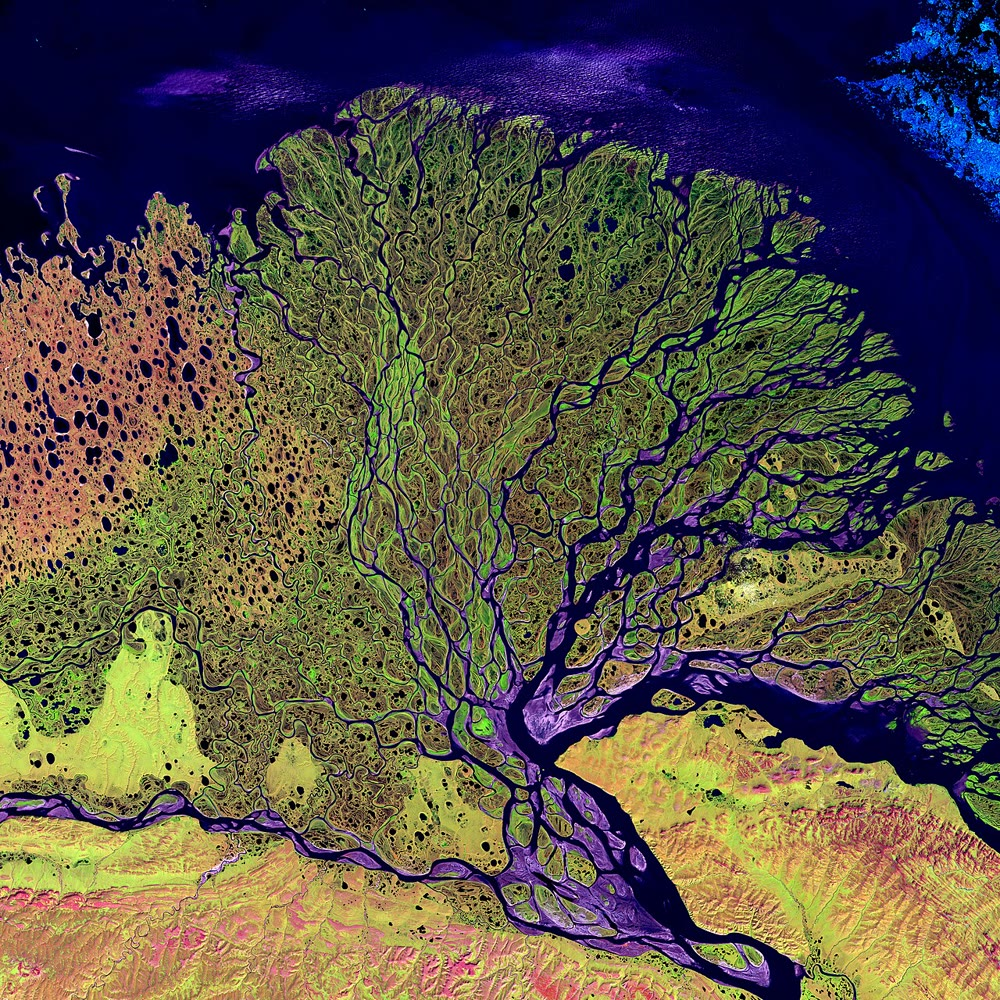
\includegraphics[width=\linewidth]{images/book1/g9-lena-delta.jpg}
\end{minipage}\hfill
\begin{minipage}[c]{0.46\linewidth}\raggedright
{\small \omterm{def:g5:water-shapes-the-land:delta}{Delta} \omterm{def:g1:landscapes-around-us:water}{Sungai} Lena, di Siberia, tempat \omterm{def:g1:landscapes-around-us:water}{sungai} itu bertemu dengan
\omterm{def:g2:water-on-earth:ocean}{Samudra} Arktik: citra Landsat warna semu tanggal 27~Februari 2000, yang
dibuat dengan inframerah gelombang pendek, inframerah, dan cahaya merah.
Banyak alur \omterm{def:g1:landscapes-around-us:water}{sungai} itu tampak berwarna biru. USGS EROS Data Center,
melalui NASA Visible Earth (domain publik, melalui Wikimedia Commons).}
\end{minipage}
% ledger: commons:lena-landsat
\label{fig:g9:maps-of-the-earth:lena}
\end{omfigure}

\section{Penentuan posisi dengan satelit}

Ponsel atau mobil dapat mengetahui letaknya sampai ketelitian beberapa
meter, hampir di mana saja di Bumi. Alat itu tidak melihat satelit; alat
itu mendengarkannya.

\begin{definition}[Penentuan posisi dengan satelit]\label{def:g9:maps-of-the-earth:positioning}
Yang disebut \emph{penentuan posisi dengan
satelit}\index{penentuan posisi dengan satelit} adalah mencari suatu posisi di Bumi dari jarak-jaraknya ke
beberapa satelit yang posisinya diketahui. Sebuah penerima menghitung
setiap jarak dari waktu yang diperlukan sinyal satelit untuk sampai
kepadanya.
\end{definition}

Sistem Amerika Serikat, GPS, mempertahankan sedikitnya 24 satelit yang
berfungsi pada \omterm{def:g4:world-physical-map:altitude}{ketinggian} sekitar \qty{20200}{km}. Setiap satelit
mengelilingi Bumi dua kali sehari, pada enam orbit yang tersebar di
sekeliling planet, sehingga dari hampir setiap titik di Bumi sedikitnya
empat satelit terlihat. Sinyal dari jarak \qty{20200}{km}, yang merambat
dengan kecepatan cahaya, tiba setelah $20\,200 \div
300\,000 \approx 0.067$~s: penerima mengukur waktu ini dan mengubahnya
menjadi jarak.
% ledger: gps:constellation, const:c (travel time computed in figdata/grade-9/trilateration.py)

Bagaimana jarak-jarak dapat memberikan posisi? Bayangkan gagasannya pada
\omterm{def:g2:drawing-to-map:map}{peta} datar. Jika penerima berjarak \qty{5}{km} dari suar~A, penerima itu
terletak di suatu tempat pada lingkaran berjari-jari \qty{5}{km} di
sekeliling A. Jika penerima itu juga berjarak \qty{10}{km} dari B,
letaknya pada kedua lingkaran itu: di salah satu dari dua titik potong
keduanya. Jarak ketiga, \qty{5}{km} dari C, memilih titik yang benar. Di
ruang angkasa, lingkaran-lingkaran itu menjadi bola, dan diperlukan satu
satelit lagi dengan alasan yang sama.

\begin{omfigure}
\begin{minipage}[c]{0.5\linewidth}\centering
\begin{tikzpicture}
\begin{axis}[x=0.42cm, y=0.42cm, xmin=-1, xmax=13, ymin=-1.5, ymax=13,
  ticks=none, axis line style={black!40}]
  \addplot[omSea!70!black, line width=0.6pt] table {figdata/out/grade-9-trilateration-circles.dat};
  \addplot[only marks, mark=triangle*, mark size=2.6pt, point meta=explicit symbolic, nodes near coords,
    nodes near coords style={font=\footnotesize\bfseries, anchor=south west, inner sep=1pt}]
    table[meta=label] {figdata/out/grade-9-trilateration-beacons.dat};
  % labels first (on a white patch), then the points on top of them
  \addplot[only marks, mark=none, point meta=explicit symbolic, nodes near coords,
    nodes near coords style={font=\footnotesize\bfseries, anchor=north east, xshift=-1pt, yshift=-1pt, inner sep=1pt, fill=white, text=red!75!black}, skip coords between index={1}{2}]
    table[meta=label] {figdata/out/grade-9-trilateration-points.dat};
  \addplot[only marks, mark=none, point meta=explicit symbolic, nodes near coords,
    nodes near coords style={font=\footnotesize, anchor=south west, xshift=1pt, yshift=1pt, inner sep=1pt, fill=white}, skip coords between index={0}{1}]
    table[meta=label] {figdata/out/grade-9-trilateration-points.dat};
  \addplot[only marks, mark=*, mark size=2pt, red!75!black, skip coords between index={1}{2}] table {figdata/out/grade-9-trilateration-points.dat};
  \addplot[only marks, mark=o, mark size=2pt, fill=white, skip coords between index={0}{1}] table {figdata/out/grade-9-trilateration-points.dat};
\end{axis}
\end{tikzpicture}
\end{minipage}\hfill
\begin{minipage}[c]{0.46\linewidth}\raggedright
{\small Penentuan posisi pada \omterm{def:g2:drawing-to-map:map}{peta} datar (sketsa; kisi dalam kilometer
tidak digambar). Penerima R berjarak \qty{5}{km} dari A, \qty{10}{km} dari
B, dan \qty{5}{km} dari C. Lingkaran di sekeliling A dan B berpotongan di
R dan di sebuah titik palsu F; hanya R yang juga terletak pada lingkaran
di sekeliling C.}
\end{minipage}
% ledger: (invented region: exercise data, figdata/grade-9/trilateration.py)
\label{fig:g9:maps-of-the-earth:trilateration}
\end{omfigure}

\begin{omfigure}
\begin{minipage}[t]{0.48\linewidth}\centering
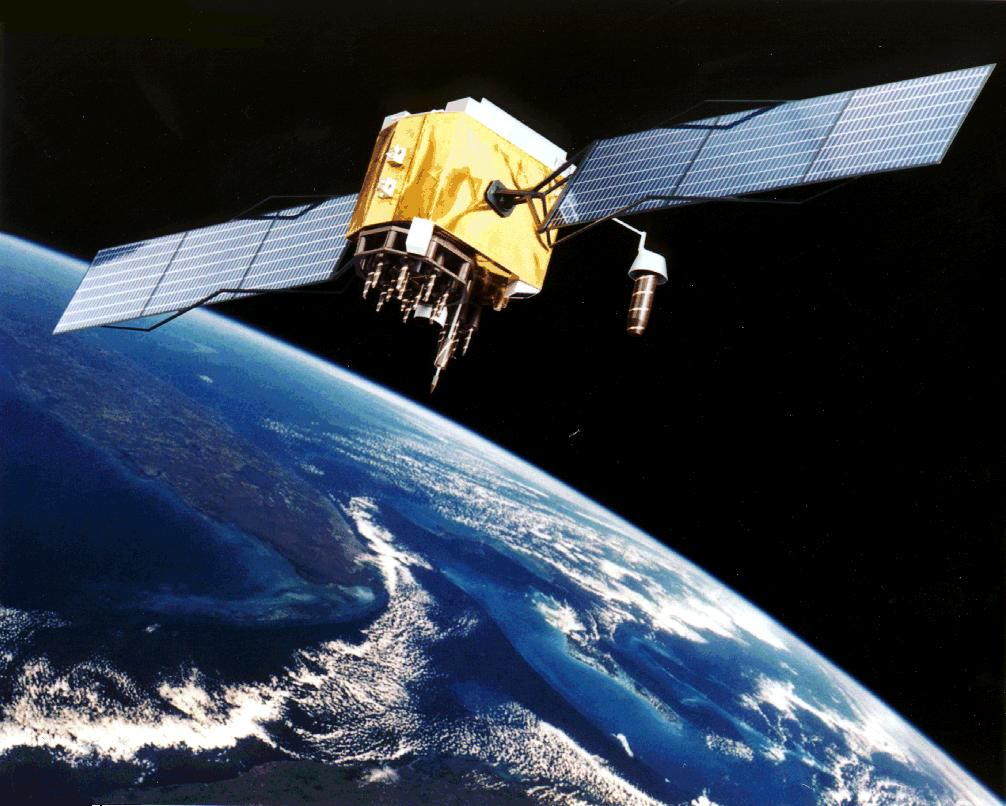
\includegraphics[width=\linewidth]{images/book1/g9-gps-satellite.jpg}

{\small Sebuah satelit GPS di orbitnya, menurut gambaran seorang seniman.
NASA (domain publik, melalui Wikimedia Commons).}
\end{minipage}\hfill
\begin{minipage}[t]{0.48\linewidth}\centering
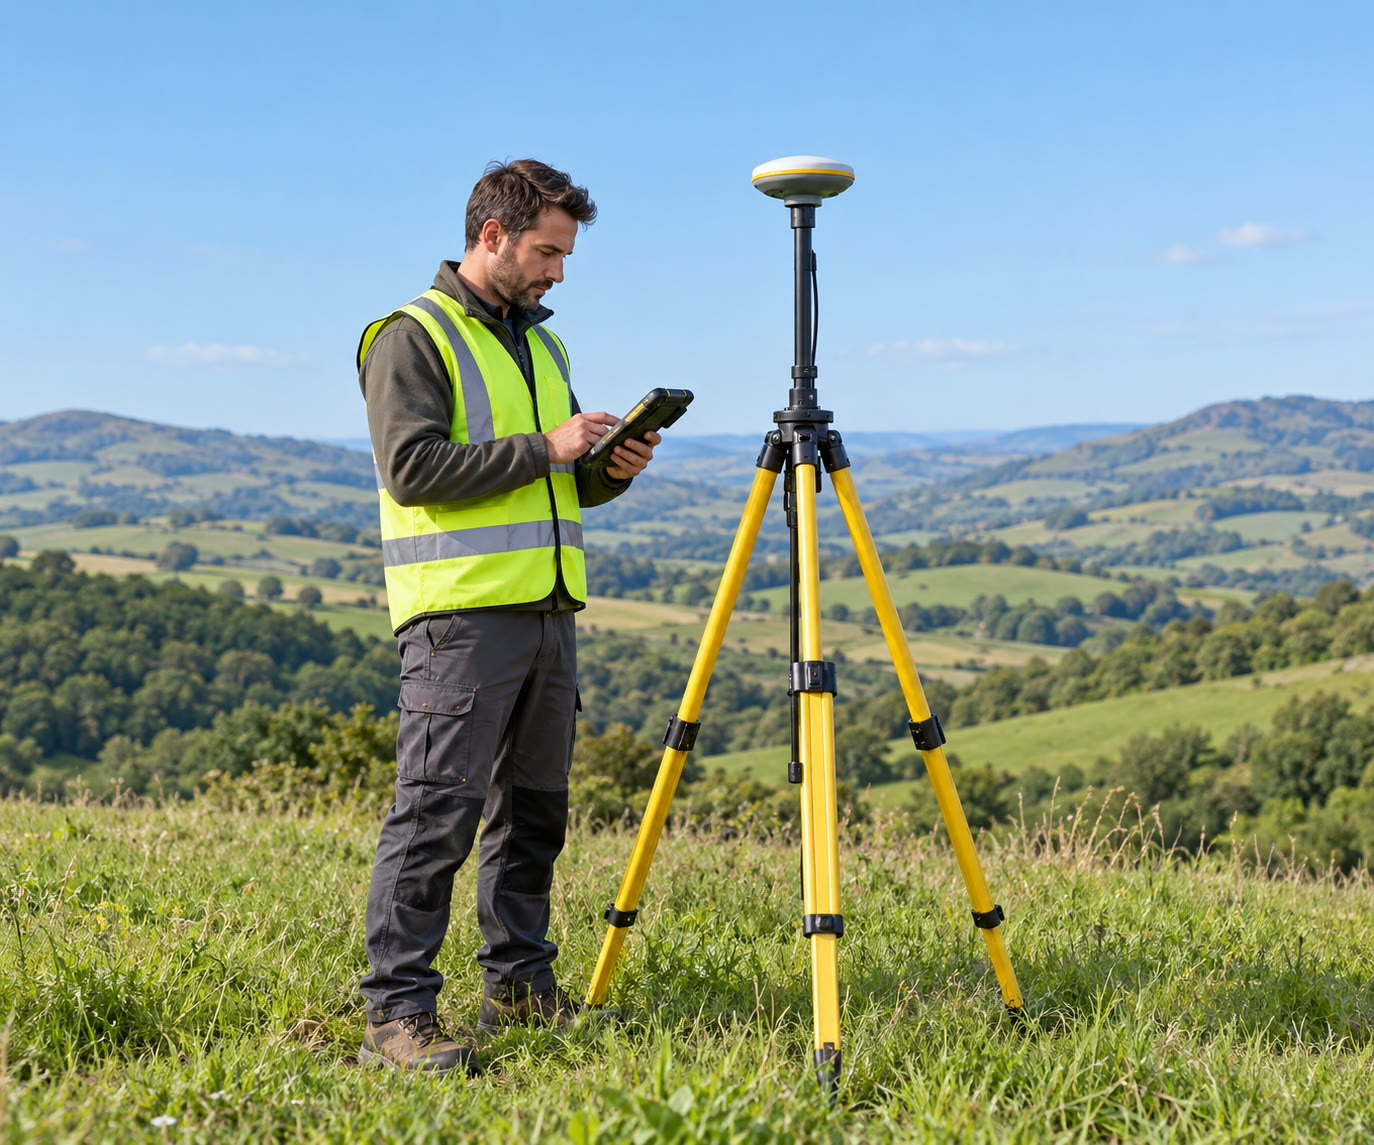
\includegraphics[width=\linewidth]{images/book1/ai/g9-surveyor.jpg}

{\small Seorang juru ukur menentukan posisi sebuah titik dengan penerima
satelit di atas tripod (ilustrasi).}
\end{minipage}
% ledger: commons:gps-iif
\label{fig:g9:maps-of-the-earth:gps}
\end{omfigure}

\section{Latihan}

\begin{exercise}[$\star$]\label{exo:g9:maps-of-the-earth:1}
Sebutkan istilah untuk setiap uraian. (a) Aturan yang memindahkan setiap
titik \omterm{def:g3:continents-and-oceans:globe}{bola dunia} ke satu titik pada \omterm{def:g2:drawing-to-map:map}{peta} datar. (b) Garis yang
menghubungkan titik-titik yang sama \omterm{def:g4:world-physical-map:altitude}{ketinggiannya}. (c) Perbandingan
seperti $1 : 50\,000$. (d) Selisih \omterm{def:g4:world-physical-map:altitude}{ketinggian} antara dua \omterm{def:g9:maps-of-the-earth:contour}{garis kontur} yang
bersebelahan. (e) Mengamati Bumi dari kejauhan, misalnya dari satelit.
\end{exercise}

\begin{exercise}[$\star$]\label{exo:g9:maps-of-the-earth:2}
Ubahlah setiap jarak pada \omterm{def:g2:drawing-to-map:map}{peta} menjadi jarak di lapangan, dalam meter
atau kilometer. (a) \qty{4}{cm} pada \omterm{def:g2:drawing-to-map:map}{peta} $1 : 25\,000$. (b) \qty{3}{cm}
pada \omterm{def:g2:drawing-to-map:map}{peta} $1 : 50\,000$. (c) \qty{2.5}{cm} pada \omterm{def:g2:drawing-to-map:map}{peta} $1 : 1\,000\,000$.
(d) Pada \omterm{def:g2:drawing-to-map:map}{peta} $1 : 25\,000$, berapa sentimeter yang mewakili \qty{1}{km}?
\end{exercise}

\begin{exercise}[$\star$]\label{exo:g9:maps-of-the-earth:3}
Benar atau salah? Perbaikilah kalimat yang salah. (a) \omterm{def:g3:continents-and-oceans:world-map}{Peta dunia} dapat
menampilkan seluruh Bumi tanpa mengubah bentuk apa pun. (b) Pada \omterm{def:g2:drawing-to-map:map}{peta}
Mercator, Greenland tampak lebih besar daripada yang sebenarnya. (c) Pada
\omterm{def:g2:drawing-to-map:map}{peta} sama luas, bentuk tetap terjaga di mana-mana. (d) \omterm{def:g9:maps-of-the-earth:numerical-scale}{Batang skala} tetap
benar ketika \omterm{def:g2:drawing-to-map:map}{peta} diperbesar dengan mesin fotokopi.
\end{exercise}

\begin{exercise}[$\star$]\label{exo:g9:maps-of-the-earth:4}
Pada \omterm{def:g9:maps-of-the-earth:topographic-map}{peta topografi}, (a) apa artinya jika garis-garis kontur sangat
rapat? (b) jika berjauhan? (c) Apa yang ditunjukkan oleh garis-garis kontur
tertutup yang makin tinggi ke arah dalam? (d) Mengapa dua \omterm{def:g9:maps-of-the-earth:contour}{garis kontur}
tidak pernah dapat berpotongan?
\end{exercise}

\begin{exercise}[$\star\star$]\label{exo:g9:maps-of-the-earth:5}
% ledger: data:ne-land (factor 1/cos^2, figdata/grade-9/projections.py)
Pada \omterm{def:g2:drawing-to-map:map}{peta} Mercator, luas pada \omterm{def:g6:latitude-longitude:latitude}{lintang} \ang{60} diperbesar 4 kali, dan pada
\omterm{def:g6:latitude-longitude:latitude}{lintang} \ang{30} sekitar 1.33 kali, dibandingkan dengan \omterm{def:g3:continents-and-oceans:equator}{khatulistiwa}.
(a) Sebuah \omterm{def:g1:landscapes-around-us:water}{danau} seluas \qty{1000}{km^2} pada \ang{60}\,LU digambar pada
\omterm{def:g2:drawing-to-map:map}{peta}. Sebuah \omterm{def:g1:landscapes-around-us:water}{danau} di \omterm{def:g3:continents-and-oceans:equator}{khatulistiwa} yang digambar dengan ukuran yang sama
mempunyai luas sebenarnya berapa? (b) Dua pulau yang luas sebenarnya sama
terletak pada \ang{30} dan pada \ang{60}. Berapa kali lebih besar pulau
kedua tampak dibandingkan dengan pulau pertama? (c) Mengapa \omterm{def:g2:drawing-to-map:map}{peta} Mercator
tidak pernah dapat menampilkan \omterm{def:g3:continents-and-oceans:poles}{kutub}?
\end{exercise}

\begin{exercise}[$\star\star$]\label{exo:g9:maps-of-the-earth:6}
% ledger: (invented region: the Varden Hills map of the chapter)
Gunakan \omterm{def:g9:maps-of-the-earth:topographic-map}{peta topografi} Perbukitan Varden dalam bab ini. (a) Berapa
\omterm{def:g9:maps-of-the-earth:contour}{interval konturnya}? (b) Berapa \omterm{def:g4:world-physical-map:altitude}{ketinggian} puncak yang ditandai dengan
titik \omterm{def:g4:world-physical-map:altitude}{ketinggiannya}, dan berapa \omterm{def:g4:world-physical-map:altitude}{ketinggian} kontur indeks yang tepat
mengelilinginya? (c) \omterm{def:g1:landscapes-around-us:water}{Sungai} mengalir ke timur. Apakah dasar \omterm{def:g1:landscapes-around-us:landform}{lembahnya} lebih
tinggi di bagian barat atau di bagian timur \omterm{def:g2:drawing-to-map:map}{peta}? (d) Di sepanjang C--D,
di sebelah utara \omterm{def:g1:landscapes-around-us:water}{sungai}, di antara garis-garis kontur yang mana
garis-garisnya paling rapat? Apa yang diceritakannya tentang kemiringan
lereng di sana?
\end{exercise}

\begin{exercise}[$\star\star$]\label{exo:g9:maps-of-the-earth:7}
% ledger: (invented region: profile C--D, figdata/grade-9/varden_topo.py)
Gunakan profil C--D dalam bab ini. (a) Pada \omterm{def:g4:world-physical-map:altitude}{ketinggian} sekitar berapa C
dan D berada? (b) Berapa \omterm{def:g4:world-physical-map:altitude}{ketinggian} terendah di sepanjang profil, dan
berapa jauh tempat itu dari C? (c) Berapa panjang dasar \omterm{def:g1:landscapes-around-us:landform}{lembah} yang datar
di sepanjang C--D? (d) Profil itu digambar dengan skala tegak yang
diregangkan tiga kali. Mengapa pembuat \omterm{def:g2:drawing-to-map:map}{peta} sering melakukan hal ini?
\end{exercise}

\begin{exercise}[$\star\star$]\label{exo:g9:maps-of-the-earth:8}
Pada \omterm{def:g2:drawing-to-map:map}{peta} $1 : 25\,000$, sebuah jalan setapak melintasi kontur
\qty{200}{m}, lalu kontur \qty{300}{m}, \qty{2}{cm} lebih jauh. (a) Berapa
jarak mendatar antara kedua titik itu di lapangan? (b) Berapa meter jalan
itu naik? (c) Berapa kemiringannya, dalam persen? (d) Lebih jauh lagi,
dua kontur yang \omterm{def:g4:world-physical-map:altitude}{ketinggiannya} berselisih \qty{100}{m} berjarak \qty{4}{cm}
pada \omterm{def:g2:drawing-to-map:map}{peta}. Apakah jalan itu lebih curam atau lebih landai di sana? Seberapa
besar bedanya?
\end{exercise}

\begin{exercise}[$\star\star$]\label{exo:g9:maps-of-the-earth:9}
% ledger: usgs:landsat1
Landsat~1 mengelilingi Bumi 14 kali sehari dan melintas di atas tempat
yang sama setiap 18 hari. (a) Berapa kali satelit itu mengorbit di antara
dua lintasan di atas tempat yang sama? (b) Setiap orbit memakan waktu 103
menit. Berapa jam lamanya 14 orbit? (c) Satelit yang dibuat untuk bekerja
satu tahun ini dimatikan pada 6~Januari 1978, lima setengah tahun setelah
peluncurannya. Berapa kali masa kerja yang direncanakan satelit itu
bekerja? (d) Sebutkan satu perubahan di permukaan Bumi yang dapat
ditunjukkan oleh citra tempat yang sama yang diambil dengan selang
bertahun-tahun.
\end{exercise}

\begin{exercise}[$\star\star$]\label{exo:g9:maps-of-the-earth:10}
% ledger: gps:constellation, const:c
Sebuah satelit GPS berjarak sekitar \qty{20200}{km}; sinyalnya merambat
sekitar \qty{300000}{km} per detik. (a) Berapa lama sinyal itu sampai?
Tuliskan jawabannya dalam notasi ilmiah. (b) Jika jam sebuah penerima
meleset $1 \times 10^{-3}$~s, berapa kesalahan jarak yang ditimbulkannya?
(c) Apa yang diceritakan hal ini tentang jam yang dipakai dalam \omterm{def:g9:maps-of-the-earth:positioning}{penentuan
posisi dengan satelit}?
\end{exercise}

\begin{exercise}[$\star\star\star$]\label{exo:g9:maps-of-the-earth:11}
Pada \omterm{def:g2:drawing-to-map:map}{peta} datar yang berkisi dalam kilometer, suar A berada di $(0, 0)$
dan suar B di $(10, 0)$. Sebuah penerima berjarak \qty{6}{km} dari A dan
\qty{8}{km} dari B. (a) Tunjukkan bahwa titik $(3.6, 4.8)$ berjarak
\qty{6}{km} dari A dan \qty{8}{km} dari B. (b) Sebutkan titik lain yang
jaraknya sama dari A dan B. (c) Suar ketiga, C, berada di $(0, 10)$, dan
penerima itu berjarak sekitar \qty{6.3}{km} darinya. Titik yang mana
letak penerima itu? (d) Mengapa \omterm{def:g9:maps-of-the-earth:positioning}{penentuan posisi dengan satelit} memerlukan
beberapa satelit?
\end{exercise}

\begin{exercise}[$\star\star\star$]\label{exo:g9:maps-of-the-earth:12}
% ledger: data:ne-land (areas, figdata/grade-9/projections.py)
Daratan utama Afrika meliputi sekitar 29~juta~\unit{km^2} dan Greenland
sekitar 2.1~juta~\unit{km^2}. (a) Berapa kali lebih luas Afrika? (b) Pada
\omterm{def:g2:drawing-to-map:map}{peta} Mercator, luas di dekat bagian tengah Greenland, pada sekitar
\ang{72}\,LU, diperbesar sekitar 10.5 kali. Perkirakan luas yang tampaknya
dimiliki Greenland. (c) Afrika terbentang melintasi \omterm{def:g3:continents-and-oceans:equator}{khatulistiwa}, tempat
luas hanya sedikit diperbesar. Bandingkan jawabanmu untuk (b) dengan luas
Afrika, lalu jelaskan \omterm{def:g2:drawing-to-map:map}{peta} dinding di awal bab ini. (d) Proyeksi mana yang
akan kamu pilih untuk menampilkan luas \omterm{def:g3:continents-and-oceans:continent}{benua-benua} secara adil?
\end{exercise}

\section{Soal: Jalan Setapak melintasi Perbukitan Varden}

\begin{problem}[{Soal akhir pekan --- para perencana telah menggambar
sebuah jalan setapak melintasi Perbukitan Varden pada peta topografi;
jawaban akhirnya adalah panjang jalan setapak itu dalam kilometer dan
total pendakiannya dalam meter}]
\label{pb:g9:maps-of-the-earth:1}
% ledger: (invented region: the Varden Hills, figdata/grade-9/varden_topo.py, part problem: leg lengths 3.6 / 2.5 / 2.35 cm, spot heights 296 / 143 / 335 / 544 m, 4.2 km, 401 m)
Jalan setapak itu berawal di sebuah rumah tani S, menurun ke sebuah
jembatan B di atas \omterm{def:g1:landscapes-around-us:water}{sungai}, lalu mendaki ke sebuah pondok W dan terus ke
puncak T. Setiap ruasnya lurus dan hanya menurun atau hanya mendaki.
\omterm{def:g2:drawing-to-map:map}{Petanya} berskala $1 : 50\,000$; \omterm{def:g4:world-physical-map:altitude}{ketinggian} S, B, W, dan T tertulis di
sampingnya.

\begin{omfigure}
\begin{tikzpicture}
\begin{axis}[x=1.6cm, y=1.6cm, xmin=2, xmax=8, ymin=1.8, ymax=6.2, ticks=none,
  axis line style={black!60}, clip mode=individual]
  \addplot[contour] table {figdata/out/shared-region-contours.dat};
  \addplot[index contour] table {figdata/out/shared-region-index-contours.dat};
  \addplot[river] table {figdata/out/shared-region-river.dat};
  \addplot[only marks, mark=none, point meta=explicit symbolic, nodes near coords,
    nodes near coords align={center}, nodes near coords style={font=\tiny, fill=white, inner sep=0.6pt, text=omContour}]
    table[meta=label] {figdata/out/grade-9-varden_topo-labels.dat};
  \addplot[red!75!black, line width=1pt, dashed] table[x=x_km, y=y_km] {figdata/out/grade-9-varden_topo-path.dat};
  \addplot[only marks, mark=*, mark size=1.6pt, red!75!black, point meta=explicit symbolic, nodes near coords,
    nodes near coords align={right}, nodes near coords style={font=\scriptsize\bfseries, text=black, fill=white, fill opacity=0.8, text opacity=1, inner sep=1pt}]
    table[meta=label] {figdata/out/grade-9-varden_topo-points.dat};
  \coordinate (na) at (axis cs:8.35,5.4);
\end{axis}
\pic at (na) {northarrow};
\end{tikzpicture}

{\small Jalan setapak S--B--W--T pada \omterm{def:g9:maps-of-the-earth:topographic-map}{peta topografi} Perbukitan Varden
(di sini diperkecil; pada \omterm{def:g2:drawing-to-map:map}{peta} aslinya, yang berskala $1 : 50\,000$,
panjang ruas-ruasnya 3.6, 2.5, dan \qty{2.35}{cm}).}
\label{fig:g9:maps-of-the-earth:path}
\end{omfigure}

\noindent\textbf{Bagian I --- Rute pada peta.}\par\nopagebreak
\begin{enumerate}[beginpenalty=10000]
  \item Dengan \omterm{def:g2:drawing-to-map:scale}{skala} $1 : 50\,000$, \qty{1}{cm} pada \omterm{def:g2:drawing-to-map:map}{peta} mewakili berapa
        meter di lapangan?
  \item Pada \omterm{def:g2:drawing-to-map:map}{peta} aslinya, ruas S--B panjangnya \qty{3.6}{cm}. Berapa
        panjangnya di lapangan, dalam kilometer?
  \item Ruas B--W dan W--T panjangnya \qty{2.5}{cm} dan \qty{2.35}{cm}.
        Berapa panjang keduanya di lapangan?
  \item Ke arah umum mana jalan itu berjalan dari B ke T?
\end{enumerate}

\noindent\textbf{Bagian II --- Pendakian.}\par\nopagebreak
\begin{enumerate}[resume, beginpenalty=10000]
  \item Berapa \omterm{def:g9:maps-of-the-earth:contour}{interval kontur} \omterm{def:g2:drawing-to-map:map}{peta} itu?
  \item Ruas mana yang menurun? Berapa meter turunnya?
  \item Berapa meter jalan itu mendaki pada ruas B--W, dan pada W--T?
  \item Berapa kemiringan rata-rata ruas W--T, dalam persen?
  \item Mengapa para perencana tidak menggambar jalan itu berupa garis
        lurus dari S ke T?
\end{enumerate}

\noindent\textbf{Bagian III --- Perjalanan kaki.}\par\nopagebreak
\begin{enumerate}[resume, beginpenalty=10000]
  \item Misalkan seorang pejalan kaki menempuh \qty{4}{km} per jam di
        tanah datar dan memerlukan satu menit tambahan untuk setiap
        \qty{10}{m} pendakian. Berapa lama seluruh perjalanan itu?
  \item Seorang pejalan kaki lain menyusuri jalan setapak itu ke arah
        sebaliknya, dari T ke S. Berapa meter ia mendaki?
  \item Berapa panjang total jalan setapak itu, dalam kilometer, dan
        total pendakiannya, dalam meter?
\end{enumerate}
\end{problem}
